% 第 4 章 方法与实现
%===============================================================================
% 修改记录:
%   2026-05-05  创建
%===============================================================================

\chapter{方法与实现}
\label{ch:method}

\section{时序参数推导}
\label{sec:timing}

FSMC 的写访问周期由\texttt{ADDSET}、\texttt{DATAST} 与 \texttt{ADDHLD}
三段构成，对应的总线波形如图~\ref{fig:fsmc_write}所示。

\begin{figure}[htbp]
    \centering
    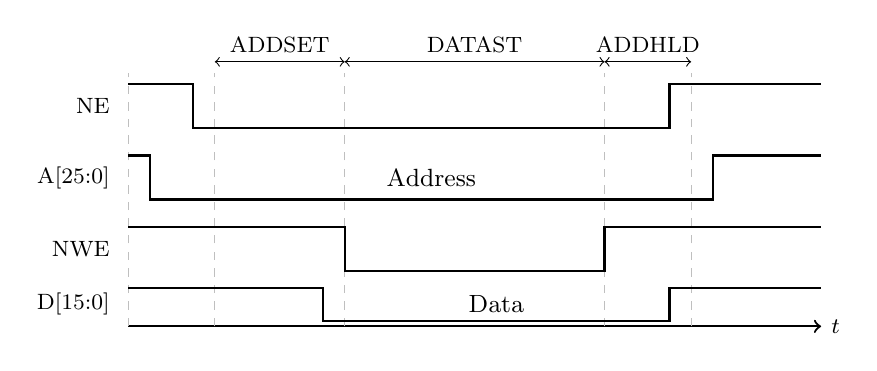
\begin{tikzpicture}[x=0.55cm, y=0.7cm, font=\footnotesize]
        % 时间轴
        \draw[->, thick] (0,0) -- (16,0) node[right] {$t$};
        \foreach \x in {0,2,5,11,13} {
            \draw[gray!50, dashed] (\x,0) -- (\x,4.6);
        }

        % 信号 NE（片选，低有效）
        \node[anchor=east] at (-0.2,4.0) {NE};
        \draw[thick] (0,4.4) -- (1.5,4.4) -- (1.5,3.6) -- (12.5,3.6) -- (12.5,4.4) -- (16,4.4);

        % 信号 A[]
        \node[anchor=east] at (-0.2,2.7) {A[25:0]};
        \draw[thick] (0,3.1) -- (0.5,3.1) -- (0.5,2.3) -- (13.5,2.3) -- (13.5,3.1) -- (16,3.1);
        \node at (7,2.7) {\small Address};

        % 信号 NWE
        \node[anchor=east] at (-0.2,1.4) {NWE};
        \draw[thick] (0,1.8) -- (5,1.8) -- (5,1.0) -- (11,1.0) -- (11,1.8) -- (16,1.8);

        % 信号 D[]
        \node[anchor=east] at (-0.2,0.4) {D[15:0]};
        \draw[thick] (0,0.7) -- (4.5,0.7) -- (4.5,0.1) -- (12.5,0.1) -- (12.5,0.7) -- (16,0.7);
        \node at (8.5,0.4) {\small Data};

        % 时序段标注
        \draw[<->] (2,4.8) -- (5,4.8) node[midway, above] {ADDSET};
        \draw[<->] (5,4.8) -- (11,4.8) node[midway, above] {DATAST};
        \draw[<->] (11,4.8) -- (13,4.8) node[midway, above] {ADDHLD};
    \end{tikzpicture}
    \caption{FSMC SRAM 异步写访问时序}
    \label{fig:fsmc_write}
\end{figure}

设系统时钟 HCLK 周期为 $T_\text{HCLK}$，则一次写访问的总周期 $T_\text{wr}$
满足：

\begin{equation}
    T_\text{wr} = (\text{ADDSET} + \text{DATAST} + \text{ADDHLD} + 1) \cdot T_\text{HCLK}
    \label{eq:twr}
\end{equation}

为保证目标 SRAM 正常工作，须同时满足三个外设侧约束：地址建立时间
$t_\text{AS} \le \text{ADDSET} \cdot T_\text{HCLK}$、写脉宽
$t_\text{WP} \le \text{DATAST} \cdot T_\text{HCLK}$、地址保持
$t_\text{AH} \le \text{ADDHLD} \cdot T_\text{HCLK}$。其中 $t_\text{AS}$、
$t_\text{WP}$、$t_\text{AH}$ 由外设手册给出。

\section{自适应时序参数搜索}
\label{sec:adaptive}

厂家推荐配置出于稳定性考虑通常预留较大裕量，导致访问周期偏长。本文
设计了一种自适应搜索方法，从厂家推荐值出发逐参数收紧，并以 64~KB 写读
校验作为正确性判据，主流程如图~\ref{fig:flow_main}所示。

\begin{figure}[htbp]
    \centering
    \begin{tikzpicture}[node distance=1.0cm and 1.6cm]
        \node[flow/start]                              (start)  {开始};
        \node[flow/proc, below=of start]               (init)   {载入厂家推荐\\ 时序参数};
        \node[flow/proc, below=of init]                (test)   {写读 64~KB\\ 校验};
        \node[flow/decide, below=of test, yshift=-0.2cm] (chk)  {校验通过?};
        \node[flow/proc, below=of chk, yshift=-0.3cm]  (down)   {DATAST $-$ 1};
        \node[flow/proc, right=2.4cm of down]          (back)   {DATAST $+$ 1\\ 锁定};
        \node[flow/start, below=of back]               (end)    {结束};

        \draw[flow/arrow] (start) -- (init);
        \draw[flow/arrow] (init)  -- (test);
        \draw[flow/arrow] (test)  -- (chk);
        \draw[flow/arrow] (chk)   -- node[right] {是} (down);
        \draw[flow/arrow] (down.west) -- ++(-1.4,0) |- (test.west);
        \draw[flow/arrow] (chk)   -- node[above] {否} (back);
        \draw[flow/arrow] (back)  -- (end);
    \end{tikzpicture}
    \caption{自适应时序参数搜索流程}
    \label{fig:flow_main}
\end{figure}

具体实现中，\texttt{DATAST} 取值从 $D_0=9$ 开始，每轮自减 1，写满 64~KB
后逐字节读回校验。一旦发现错误，立刻回退一拍并锁定。\texttt{ADDSET} 与
\texttt{ADDHLD} 的处理类似。该方法不依赖具体外设型号，可在程序启动时
自动完成参数调优，避免人工查表。
